\beginsong{An den sechs vergang'nen Tagen}[
    wuw={Alf Zschiesche}, 
    bo={26}, 
    pfii={28}, 
    pfiii={55}, 
    gruen={58}, 
    siru={18},
    tonspur={148},
]

\beginverse*
\nolyrics
\[C] \[Fm] \[G] \[C] \echo{Sarah Connor} \rep{2}
\[C] \[G/h] \[B&] \[A]
\endverse

\beginverse
\endverse
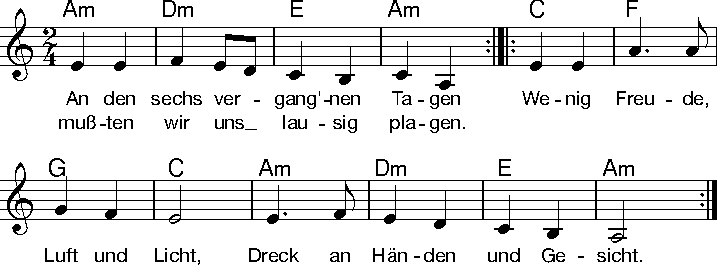
\includegraphics[draft=false, width=1\textwidth]{Noten/Lied102.pdf}

\beginverse\memorize
\[Am]Heute \[Dm]hat die \[E]Welt uns \[Am]wieder, Klampfen\[Dm]spiel und \[E]hundert \[Am]Lieder,
\lrep \[C]wandern \[F]durch die \[G]Wälder \[C]mit \[Am]zu dem \[Dm]Sieben\[E]meilen\[Am]schritt. \rrep
\endverse

\beginverse*
\nolyrics
Bond-Theme: \[Am] \rep{8}
\endverse

\beginverse
^Und so ^geht es ^immer ^munter Berge ^rauf und ^wieder ^runter,
\lrep ^alle ^uns're ^Müdig^keit ^steckt zu^haus im ^Arbeits^kleid. \rrep
\endverse

\beginverse*
\nolyrics
Drums \echo{8 Takte}
Drums, Posaune, Sax, Bass: \[Am] \echo{8 Takte}
\endverse

\beginverse 
^ \[-]Sieben Tage hat die Woche, \[Am]sechse \[Dm]sind wir \[E]rumge\[Am]krochen,
\lrep \[C]doch am \[F]siebten \[G]lebt sich's \[C]flott, \[Am]also \[Dm]will's der \[E]liebe \[Am]Gott. \rrep
\endverse

\endsong
